%% LyX 2.1.4 created this file.  For more info, see http://www.lyx.org/.
%% Do not edit unless you really know what you are doing.
\documentclass[english]{article}
\usepackage[T1]{fontenc}
\usepackage[utf8]{luainputenc}
\setlength{\parskip}{\smallskipamount}
\setlength{\parindent}{0pt}
\usepackage{graphicx}
\PassOptionsToPackage{normalem}{ulem}
\usepackage{ulem}

\makeatletter
%%%%%%%%%%%%%%%%%%%%%%%%%%%%%% User specified LaTeX commands.
\date{}

\makeatother

\usepackage{babel}
\begin{document}

\title{EEGLAB SPoC plug-in tutorial}

\maketitle

\section*{What is the SPoC plug-in for EEGLAB?}

The SPoC plug-in is a set of Matlab tools developed by the IDA group
of the TU of Berlin, that allows the decomposition of the EEG data
using the SSD, SPoC and cSPoC methods. These tools are designed to
work within the EEGLAB environment, providing a GUI to decompose the
data into different relevant components:
\begin{enumerate}
\item SSD - Extracts components with optimized signal-to-noise ratio at
a frequency band of interest.
\item SPoC - Extracts components with maximal power covariance with the
univariate target function z.
\item cSPoC - Extracts components with maximal envelope correlations from
N oscillatory and multivariate datasets. For N>2, the extracted components
maximize the pairwise averaged envelope correlations.
\end{enumerate}
All of the tools can also be used from the Matlab command line, providing
expert users with the ability to use them in custom scripts.


\section*{Requirements}

In addition to the requirements of EEGLAB, SPoC plug-in requires the
following folders to be stored in the plug-in folder: \textbf{SSD
; SPoC ; cSPoC ; utils}. These folders are found in the following
repository:

\textit{https://github.com/svendaehne/matlab\_SPoC.}


\section*{Download and Installation}
\begin{enumerate}
\item Go to:


\textit{https://github.com/svendaehne/eeglab\_plugins}


push the ``Download ZIP'' botton and choose where to save the file.

\item Uncompress the downloaded file into the 'plugins' directory of your
EEGLAB distribution. You should now have a directory called 'SPoC'
containing necessary files.
\item Obtain the following folders from the SPoC repository


\textit{(https://github.com/svendaehne/matlab\_SPoC)}


and store them in the 'SPoC' directory: \textbf{SSD, SPoC, cSPoC,
utils}.

\end{enumerate}
Starting EEGLAB should now automatically recognize and add the plug-in.
You should see the following line appear in your Matlab environment
window:

EEGLAB: adding \textquotedbl{}SPoC\textquotedbl{} v.1.0 (see >\textcompwordmark{}>
help eegplugin\_AD)
\begin{description}
\item [{Voilà!}]~
\end{description}

\section*{Tutorial}


\subsection*{Using components}

After running each of these decompositions your data will be assigned
with components. These components are saved in the ICA components
slot (EEG.icaweights).

Read the ICA tutorial

(\textit{http://sccn.ucsd.edu/wiki/Chapter\_09:\_Decomposing\_Data\_Using\_ICA})

to learn about the following actions which can be performed using
AD components, in the exact same manner:
\begin{enumerate}
\item Plotting scalp maps


(\textit{http://sccn ... \#Plotting\_2-D\_Component\_Scalp\_Maps})

\item Plotting components activation


(\textit{http://sccn ... \#Scrolling\_through\_component\_activations})

\item Studying and removing components


(\textit{http://sccn ... \#Studying\_and\_removing\_ICA\_components})

\end{enumerate}

\subsection*{SSD}

The SSD function extracts components with optimized signal-to-noise
ratio at a frequency band of interest.


\subsubsection*{Preparation}
\begin{enumerate}
\item Run EEGLAB and load the relevant dataset/s. Data can be either epochs
or continuous EEG.
\end{enumerate}

\subsubsection*{Run}
\begin{enumerate}
\item Select \textbf{Tools > SPoC > Run SSD}. This calls the function pop\_ssd.m.


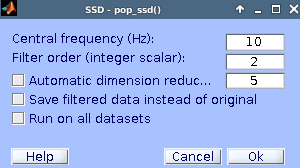
\includegraphics[scale=0.7]{pics/ssd_form_e}

\item Fill out the parameters form and press \textbf{OK}. Here is the parameters
description (top down, left to right):

\begin{enumerate}
\item Central frequency for the filtering processes. The calculation of
the cut-off frequencies is as follows:

\begin{enumerate}
\item signal band-pass$=2^{(log2(fc)-0.25)};2^{(log2(fc)+0.25)}$.
\item noise band-past$=2^{(log2(fc)-0.9)};2^{(log2(fc)+0.9)}$.
\item noise band-stop$=2^{(log2(fc)-0.35)};2^{(log2(fc)+0.35)}$.
\end{enumerate}

'fc' being the chosen central frequency.

\item Filter order used for butterworth bandpass and bandstop filtering.
If unsure about it, use the default value of order 2.
\item Automatically subtract components from data (Yes/No).
\item Numbers of component to keep (the rest will be subtracted). Only relevant
if you marked the checkbox in (c).
\item Overwrite the original data with the data filtered around the central
frequency given at (a) (Yes/No). Notice that after running this option,
the original data will be lost if not saved separately!
\item Run the same calculation on all loaded datasets (Yes/No).
\end{enumerate}

In case the data is continues and contains event marks, you could
also choose to use only event related data:


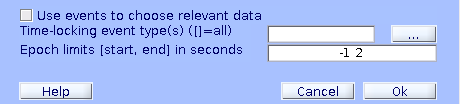
\includegraphics[scale=0.7]{pics/ssd_form_c}
\begin{enumerate}
\item Mark to use this option.
\item The name of the event/s you wish to use.
\item The limits around the events. Data outside these limits will not be
taken into account for the calculation.
\end{enumerate}
\item Wait until the following massage (With your dataset name) appears
and press \textbf{OK}.


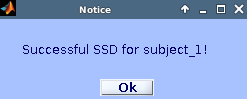
\includegraphics[scale=0.7]{pics/ssd_s}

\end{enumerate}
The components spatial filters are now stored under EEG.icaweights
while old weights from pervious decompositions are stored under EEG.etc.oldweights.

In the structure EEG.dipfit.model you can find the lambda values.


\subsubsection*{Plot}

For SSD and SPoC you can plot the lambda values of the decomposition.
Select \textbf{Plot > SPoC > Lambda spectrum}.

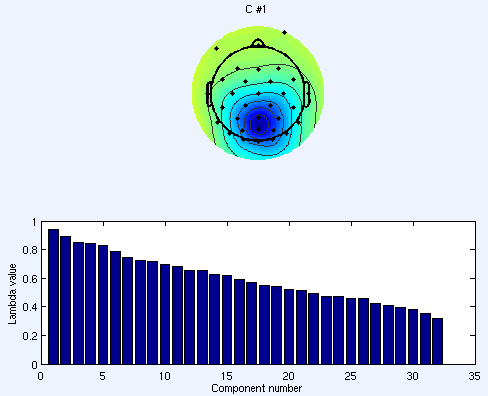
\includegraphics[scale=0.7]{pics/lambda_plot}

clicking on a blue bar shows the scalp plot of the relevant component. 


\subsection*{SPoC}

The SPoC function extracts components with maximal power covariance
with the univariate target function z.


\subsubsection*{Preparation}

To get the best results we recommend applying SPoC analysis only after
\uline{filtering} and \uline{reducing data dimension} using
SSD. To do both, select \textbf{Tools > SPoC > Run SSD}, mark the
``\textbf{Dimension reduction}'' and ``\textbf{Save filtered data
instead of original}'' checkboxes and choose the relevant central
frequency and the number of components you wish to keep (=dimension
degree).
\begin{enumerate}
\item Save the relevant target function z as a vector in a .mat file.
\item Run EEGLAB and load the relevant dataset. Data can be either epochs
or continuous EEG. In the continues case data will be segmented based
on its events. Make sure that the number of epochs or events is equal
to the length of your target function z vector.
\end{enumerate}

\subsubsection*{Run}
\begin{enumerate}
\item Select \textbf{Tools > SPoC > Run SPoC}. This calls the function pop\_spoc.m.


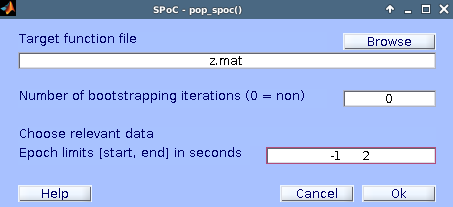
\includegraphics[scale=0.7]{pics/spoc_form_e}

\item Fill out the parameters form and press \textbf{OK}. Here is the parameters
description (top down, left to right):

\begin{enumerate}
\item Target function z file path. You could use the browse option to find
the file in your folders.
\item Number of bootstrapping iterations used to calculate p-values of the
results.
\item The relevant data limits for the calculation. Data outside these limits
will not be taken into account for the calculation.
\end{enumerate}

In case the data is continues, you could still use SPoC based on event
marks:


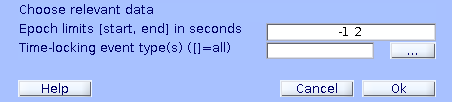
\includegraphics[scale=0.7]{pics/spoc_form_c}
\begin{enumerate}
\item The limits around the events. Data outside these limits will not be
taken into account for the calculation.
\item The name of the event/s you wish to use.
\end{enumerate}
\item Wait until the following massage (With your dataset name) appears
and press \textbf{OK}.


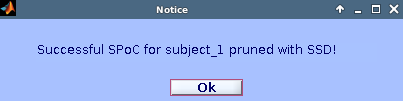
\includegraphics[scale=0.7]{pics/spoc_s}

\end{enumerate}
The components spatial filters are now stored under EEG.icaweights
while old weights from pervious decompositions are stored under EEG.etc.oldweights.

In the structure EEG.dipfit.model you can find the lambda values,
p values and the SPoC signal function of each component.


\subsubsection*{Plot}

See the plot section of SSD for lambda spectrum plot.

Select \textbf{Plot > SPoC > SPoC results}.

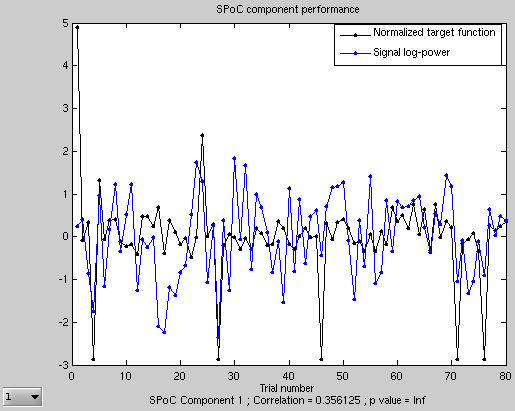
\includegraphics[scale=0.6]{pics/spoc_plot}

Choose any component from the drop list to show its power function
next to the target function. 


\subsection*{cSPoC}

The cSPoC function extracts components with maximal envelope correlations
from N oscillatory and multivariate datasets. For N>2, the extracted
components maximize the pairwise averaged envelope correlations.


\subsubsection*{Preparation}

To get the best results we recommend applying cSPoC analysis only
after \uline{filtering} and \uline{reducing data dimension}
using SSD. To do both, select \textbf{Tools > SPoC > Run SSD}, mark
the ``\textbf{Dimension reduction}'', ``\textbf{Save filtered data
instead of original}'' and ``\textbf{Run on all datasets}'' checkboxes
and choose the relevant central frequency and the number of components
you wish to keep (=dimension degree).
\begin{enumerate}
\item Run EEGLAB and load all relevant datasets. Any loaded dataset will
be taken into account. Make sure that all datasets are segmented to
the same number of epochs.
\end{enumerate}

\subsubsection*{Run}
\begin{enumerate}
\item Select \textbf{Tools > SPoC > Run cSPoC}. This calls the function
pop\_cspoc.m.


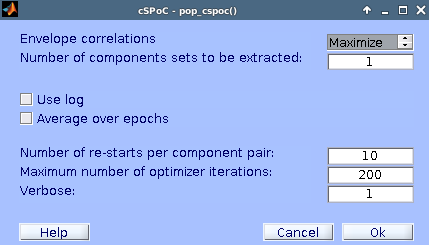
\includegraphics[scale=0.7]{pics/cSPoC_form}

\item Fill out the parameters form and press \textbf{OK}. Here is the parameters
description (top down, left to right):

\begin{enumerate}
\item Maximizing or minimizing the envelopes correlation.
\item Number of envelope-correlated components per dataset to be extracted.
\item Optimize correlations of log-envelopes rather then envelopes (Yes/No).
\item When optimizing the correlations, average the source envelopes within
epochs (Yes/No).
\item Number of re-starts per component pair.
\item Maximum number of optimizer iterations.
\item Level of detail in command line output.
\end{enumerate}
\item Wait until the following massage appears and press \textbf{OK}.


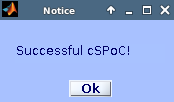
\includegraphics[scale=0.7]{pics/cspoc_s}

\end{enumerate}
The components spatial filters are now stored under EEG.icaweights
while old weights from pervious decompositions are stored under EEG.etc.oldweights.

In the structure EEG.dipfit.model you can find all the correlation
r values.


\subsubsection*{Plot}

Select \textbf{Plot > SPoC > cSPoC results}.

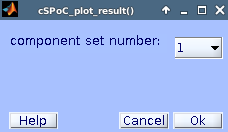
\includegraphics[scale=0.7]{pics/cspoc_plot_form}

In the pop-up window, select which component set you would like to
plot.

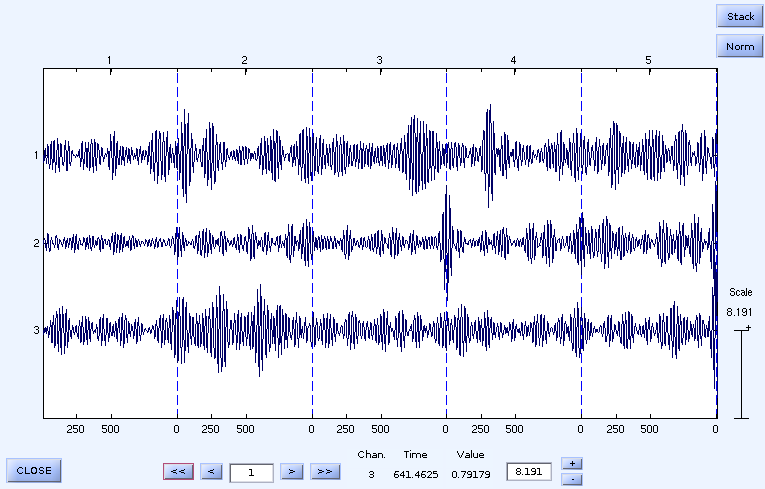
\includegraphics[scale=0.4]{pics/cspoc_plot}

We recommend increasing the displayed number of epochs using \textbf{Setting
> Time range to display > Number of epoch(s)}.
\begin{thebibliography}{1}
\bibitem{key-1}Nikulin VV, Nolte G, Curio G. A novel method for reliable
and fast extraction of neuronal EEG/MEG oscillations on the basis
of spatio-spectral decomposition. NeuroImage, 2011, 55: 1528-1535.

\bibitem{key-2}S. Dähne, F. C. Meinecke, S. Haufe, J. Höhne, M. Tangermann,
K. R. Müller, V. V. Nikulin, \textquotedbl{}SPoC: a novel framework
for relating the amplitude of neuronal oscillations to behaviorally
relevant parameters\textquotedbl{}, NeuroImage, 86(0):111-122, 2014

\bibitem{key-3}S. Dähne, V. V. Nikulin, D. Ramirez, P. J. Schreier,
K. R. Müller, S. Haufe, \textquotedbl{}Finding brain oscillations
with power dependencies in neuroimaging data\textquotedbl{}, NeuroImage,
96:334-348, 2014

\bibitem{key-4}S. Haufe, S. Dähne, V. V. Nikulin, \textquotedbl{}Dimensionality
reduction for the analysis of brain oscillations\textquotedbl{} NeuroImage
101:583-597 2014\end{thebibliography}

\end{document}
